% Created 2025-07-05 Sat 18:02
% Intended LaTeX compiler: pdflatex
\documentclass[11pt]{article}
\usepackage[utf8]{inputenc}
\usepackage[T1]{fontenc}
\usepackage{graphicx}
\usepackage{longtable}
\usepackage{wrapfig}
\usepackage{rotating}
\usepackage[normalem]{ulem}
\usepackage{amsmath}
\usepackage{amssymb}
\usepackage{capt-of}
\usepackage{hyperref}
\author{Tobi Lehman}
\date{\today}
\title{The God Groupoid}
\hypersetup{
 pdfauthor={Tobi Lehman},
 pdftitle={The God Groupoid},
 pdfkeywords={},
 pdfsubject={},
 pdfcreator={Emacs 30.1 (Org mode 9.7.11)}, 
 pdflang={English}}
\begin{document}

\maketitle
\tableofcontents

\section{Introduction}
\label{sec:orgdf5438b}
This is my attempt to formulate the Catholic theology of the Trinity in mathematical language. If you find any errors in the math or the theology, please email me at \url{mailto:mail@tobilehman.com}, I care deeply about getting this right. To my mathematician's eyes, the Catechism of the Catholic Church (\href{https://www.vatican.va/archive/ENG0015/\_INDEX.HTM}{CCC}) has parts that remind me of a mathematical text. The axiomatic truths asserted early on, the precise and consistent use of language, the fidelity to reason. I don't know if the entire Catechism could be written to look like a math text, or if it even should, but I think the doctrine of trinity can. This is my best attempt to do so. God bless.

For background on category theory or Catholic theology, see my \hyperref[sec:org717892e]{sources} section.
\section{Definitions}
\label{sec:orgdb00d48}
$$\begin{align}\mathcal{G} &= \text{God} \\ F &= \text{The Father}\\ S &= \text{The Son} \\ H &= \text{The Holy Spirit} \\ (X \stackrel{\dagger}{=} Y) &= (X \text{ is consubstantial with } Y) \end{align}$$
\subsection{The category \(\mathcal{G}\)}
\label{sec:orge39f9f8}

We will represent the triune God \(\mathcal{G}\) as a category where the set of objects is:

$$\text{ob}(\mathcal{G}) = \{F,S,H\}$$

\begin{center}
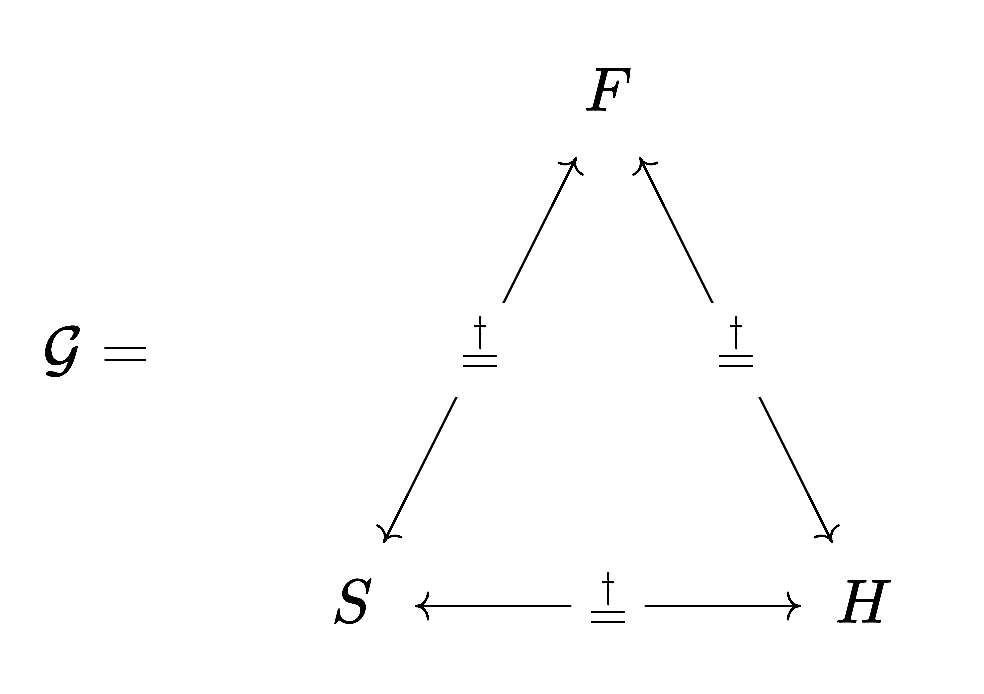
\includegraphics[width=.9\linewidth]{./trinity.png}
\end{center}

And all the sets of morphisms are isomorphisms, they are the \(\stackrel{\dagger}{=}\) relation, which is read "is consubstantial with".

$$\text{Hom}(F,S) = \{ \stackrel{\dagger}{=}_{FS} : F \to S \} $$
$$\text{Hom}(S,H) = \{ \stackrel{\dagger}{=}_{SH} : S \to H \} $$
$$\text{Hom}(H,F) = \{ \stackrel{\dagger}{=}_{HF} : H \to F \} $$
$$\text{Hom}(S,F) = \{ \stackrel{\dagger}{=}_{SF} : S \to F \} $$
$$\text{Hom}(F,H) = \{ \stackrel{\dagger}{=}_{FH} : F \to H \} $$
$$\text{Hom}(H,S) = \{ \stackrel{\dagger}{=}_{HS} : H \to S \} $$
\subsection{Interpreting "God is the Father"}
\label{sec:orgfa8d053}
Bill Clinton once reminded us that it depends on what your definition of "is" is. We have formalized the sentences like "The Father is consubstantial with the Son", but then defined God as the category that contains the Father, Son and Holy Spirit. What does it mean to say that "God is the Father" (In our notation: \(\mathcal{G}\) "is" \(F\))?
\subsubsection{The \(\text{Is}\) Functors}
\label{sec:org4c89dc1}

We interpret the sentence "God is the Father" using the

\(\text{Is}_F : \mathcal{G} \to \mathcal{G}\downarrow F\) \hyperref[sec:org5f61f9d]{Functor}.


\(\mathcal{G}\downarrow F\) is the \hyperref[sec:org31eacc6]{slice category} construction,
which makes a category out of an object that isomorphic to \(\mathbb{1}\).
\begin{enumerate}
\item Functors
\label{sec:org5f61f9d}
Given a category \(\mathcal{C}\) and a category \(\mathcal{D}\), a \textbf{\textbf{functor}} is a mapping from the objects of \(\mathcal{C}\) to the objects of \(\mathcal{D}\), such that morphism composition is preserved. So if \(f : A \to B\) is a morphism in \(\mathcal{C}\), then \(F(f) : F(A) \to F(B)\) is a morphism in \(\mathcal{D}\).
\item Slice Category
\label{sec:org31eacc6}
Given a category \(\mathcal{C}\) and an object \(c \in \text{ob}(\mathcal{C})\), the \textbf{\textbf{slice category}} \(\mathcal{C}\downarrow c\) is a category where:
\begin{itemize}
\item Objects are morphisms \(f : x \to c\) in \(\mathcal{C}\)
\item Morphisms from \(f : x \to c\) to \(g : y \to c\) are morphisms \(h : x \to y\) in \(\mathcal{C}\) such that \(g \circ h = f\)
\end{itemize}
\end{enumerate}
\subsection{Lemma 1.1: \(\mathcal{G}\) is a groupoid}
\label{sec:org2f57b60}

A \href{https://math.jhu.edu/\~eriehl/context.pdf\#page=25}{groupoid} is a category in which every morphism is an isomorphism. That's another way of saying every morphism has an inverse.
\subsubsection{Proof:}
\label{sec:org9072856}
If you look at the hom-sets above, you will see that for every \(\text{Hom}(X,Y)\) there's a \(\text{Hom}(Y,X)\).
Without loss of generality, consider \(\text{Hom}(F,S)\), which asserts that "The Father is consubstantial with The Son". 
\section{Axioms}
\label{sec:org3a83f4b}
\begin{enumerate}
\item There is one God (\href{https://www.vatican.va/archive/ENG0015/\_\_P16.HTM}{CCC:200})
\item There are three Divine Persons, The Father, The Son and The Holy Spirit. All are fully God. (\href{https://www.vatican.va/archive/ENG0015/\_\_P17.HTM}{CCC:253}).
\item The Father is consubstantial with The Son, who is consubstantial with the Holy Spirit. (\href{https://www.vatican.va/archive/ENG0015/\_\_P20.HTM}{CCC:689})
$$F \stackrel{\dagger}{=} S \stackrel{\dagger}{=} H$$
\item All things come from The Father (\href{https://www.vatican.va/archive/ENG0015/\_\_P17.HTM}{CCC:258})
$$\forall x : \text{from}_F(x)$$

\item All things are through The Son (\href{https://www.vatican.va/archive/ENG0015/\_\_P17.HTM}{CCC:258})
$$\forall x : \text{through}_S(x)$$

\item All things are in The Holy Spirit (\href{https://www.vatican.va/archive/ENG0015/\_\_P17.HTM}{CCC:258})
$$\forall x : \text{in}_H(x)$$
\end{enumerate}
\section{The Most Holy Trinity}
\label{sec:org0b54c16}
God is the Father, the Son, and the Holy Spirit. The use of the word "is" doesn't follow the same transitive rules as \(=\) in mathematics. There's another branch of math that deals with this, category theory. Category theory goes beyond the idea of "strict equality" and focuses on relationships and mappings between objects. This distinction will be useful in trying to understand the Trinity.

Let \(G = \text{God}\), \(F = \text{The Father}\), \(S = \text{The Son}\) and \(H = \text{The Holy Spirit}\).

If "is" was the normal \(=\) sign, then we could prove something false.

To avoid false arguments like the above, we have to define "Is" in a precise way.
\subsection{Definitions of "Is":}
\label{sec:org109becd}

\subsubsection{Definition of "\(\text{Divine Person}\) is God"}
\label{sec:org02b50cd}

We define the following functors:

\begin{itemize}
\item \(\text{Is}_F : \mathcal{G}\downarrow F \to \mathcal{G}\)
\item \(\text{Is}_S : \mathcal{G}\downarrow S \to \mathcal{G}\)
\item \(\text{Is}_H : \mathcal{G}\downarrow H \to \mathcal{G}\)
\end{itemize}

The way we defined \(\mathcal{G}\) means that \textbf{the whole category} is God. The objects, like \(F\) are not
equal to the whole, but they are equivalent the above precise sense.
\subsubsection{Proof that \(\text{Is}_x\) avoids the transitivity error}
\label{sec:org4b2f95e}

The \(\text{Is}_F\) functor asserts that the Father is equivalent to God.

The \(\text{Is}_S\) functor asserts that the Son is equivalent to God.

\begin{center}
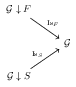
\includegraphics[width=.9\linewidth]{./no-transitive.png}
\end{center}

The diagram above says that "The Father is God" and that "The Son is God", but it does not say that
"The Father is the Son".

The Father \(F\) is \emph{consubstantial with} (\(\stackrel{\dagger}{=}\)) The Son \(S\):

$$\stackrel{\dagger}{=}_{FS} : F \to S$$

But the \(\stackrel{\dagger}{=}_{FS} : F \to S\) and \(\text{Is}_S : \mathcal{G}\downarrow S \to \mathcal{G}\) arrows
don't compose. Graphically:

\begin{center}
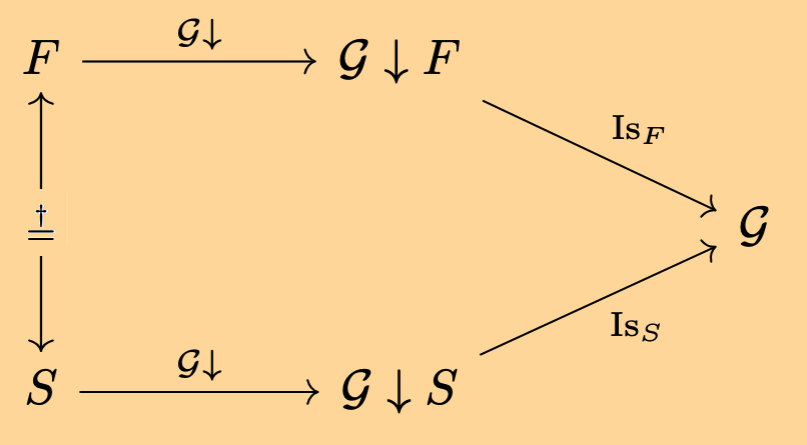
\includegraphics[width=.9\linewidth]{./f-is-not-s.png}
\end{center}

From the above diagram, you can see that you cannot find a path from \(F\) to \(S\) that goes through \(\mathcal{G}\),
this is how the above definition avoids the transitivity error.
\section{Sources}
\label{sec:org717892e}
\subsection{BCT}
\label{sec:orge9d2214}
\href{https://arxiv.org/pdf/1612.09375\#page=18}{\emph{Basic Category Theory} by Tom Leinster}
\subsection{CTIC}
\label{sec:org4989c75}
\href{https://emilyriehl.github.io/files/context.pdf}{\emph{Category Theory in Context} by Emily Riehl}
\subsection{CCC}
\label{sec:org4ae31f1}
\href{https://www.vatican.va/archive/ENG0015/\_INDEX.HTM}{\emph{Catechism of the Catholic Church}}
\end{document}
